\section{Taxonomy of Trustworthiness}

The evolution of LALMs from specialized speech recognition to complex paralinguistic reasoning necessitates a robust framework for assessing their trustworthiness in high-stakes domains. We therefore establish a systematic taxonomy organized around six analytical pillars: \textbf{hallucination}, \textbf{robustness}, \textbf{safety}, \textbf{privacy}, \textbf{fairness}, and \textbf{authentication} as shown in figure \ref{fig:3}. This multidimensional framework serves as the structural foundation of our review, allowing for a comprehensive synthesis of both offensive vulnerabilities and defensive countermeasures.

\subsection{Hallucination and Faithfulness}
Unlike text-based hallucinations that stem from parametric knowledge gaps, Audio LLM hallucinations often originate from the \textit{acoustic-semantic gap}---a disconnect between what the model acoustically perceives and what it textually generates. This manifests in several distinct failure modes.

\textbf{Modality Neglect.} A growing body of evidence suggests that current LALMs frequently default to textual shortcuts while underutilizing acoustic information. Systematic studies demonstrate that models over-rely on lexical cues rather than acoustic emotion signals \cite{chen2025audio}, and that replacing audio inputs with silence or noise causes negligible performance changes on certain benchmarks \cite{wang2025audio}. Quantitative analysis using Shapley-value-based frameworks further confirms that the text modality dominates model predictions even in ostensibly audio-centric tasks \cite{morais2025investigating}. The impact of irrelevant audio on text reasoning \cite{li2025silence} additionally reveals that extraneous acoustic information can actively degrade performance, indicating fragile audio-text integration.

\textbf{Grounding Failures.} Beyond modality neglect, LALMs exhibit failures in acoustically grounding their outputs. Research on audio geo-localization \cite{zhang2026sonar} highlights challenges where models must reason over environmental sounds without hallucinating geographic metadata. Investigations into faithfulness \cite{jain2025investigating} reveal that model outputs may be internally consistent yet factually inconsistent with the auditory input, suggesting that surface-level fluency masks deeper grounding deficits. Towards addressing these issues, reliability-oriented frameworks \cite{ma2025towards} propose systematic approaches to quantify and reduce ungrounded generations.


\textbf{Attention Rebalancing as Mitigation.} To counteract modality bias, audio-contribution-aware post-training methods dynamically rebalance modality weights \cite{he2025measuring}, while cross-modal attention mechanisms explicitly enforce the model's reliance on acoustic evidence \cite{wang2025pay}. These approaches represent a shift from post-hoc detection to architectural prevention of hallucinations.

\subsection{Robustness and Adversarial Vulnerabilities}
Robustness in the audio domain encompasses both naturally occurring environmental variations and intentionally crafted adversarial perturbations.

\textbf{Evaluation-Level Robustness.} Even under benign evaluation conditions, LALMs exhibit notable fragility. Robustness assessments under multiple-choice settings \cite{lopez2025robustness} reveal that minor perturbations to answer options or prompt phrasing can significantly alter model outputs. Instruction sensitivity benchmarks \cite{li2025isa} further demonstrate that semantically equivalent but syntactically varied prompts yield inconsistent responses, undermining deployment reliability.

\textbf{Adversarial Audio Attacks.} More concerning are intentional adversarial perturbations. Research demonstrates that imperceptible waveform modifications---``attacker's noise''---can manipulate LALMs in real-world settings \cite{sadasivan2025attacker}. Audio narrative attacks \cite{yu2026now} further exploit the sequential nature of audio to embed adversarial instructions within seemingly benign speech streams.

\textbf{Backdoor Vulnerabilities.} The integrity of LALMs is also threatened at the training level. Latent acoustic pattern triggers can be embedded during alignment to activate specific malicious behaviors upon encountering particular audio signatures \cite{lin2025hidden}. Complementary work on backdoor attacks against speech language models \cite{fortier2025backdoor} reveals that such vulnerabilities persist across different architectural paradigms. Analyzing reasoning shifts under adversarial conditions \cite{nguyen2026analyzing} reveals a ``reasoning tax'' phenomenon: defensive measures that protect against attacks simultaneously degrade the model's legitimate reasoning capabilities. Such embedded trojans typically leverage imperceptible frequency shifts or background acoustics, allowing malicious intents to remain completely dormant during standard inference. Consequently, breaking this trade-off stands as a paramount challenge for ensuring robust alignment.


\subsection{Authentication and Deepfake Detection}
The advent of high-fidelity generative speech has prompted the integration of LALMs into counter-spoofing, where their sophisticated auditory reasoning is utilized to expose subtle neural artifacts that elude traditional classifiers.

\textbf{Speaker Authentication.}
While deepfake detection aims to distinguish real from synthetic speech, speaker authentication focuses on verifying or identifying the speaker's identity. Conventional speaker verification systems rely on task-specific embedding extractors and scoring backends, but recent work has begun to reformulate speaker verification as an audio question-answering task for LALMs. Ren et al. \cite{ren2025audiolargelanguagemodels} systematically evaluate LALMs for speaker verification by prompting them with enrollment--test utterance pairs. Their results show that current LALMs exhibit limited zero-shot verification capability under challenging acoustic conditions, but lightweight supervised fine-tuning with rule-based hard pair sampling substantially improves LALMs' performance \cite{ren2025audiolargelanguagemodels}. These findings suggest that LALMs may support more flexible authentication interfaces, such as instruction-following speaker verification and joint reasoning over identity claims and acoustic evidence. However, LALM-based authentication also introduces security and privacy risks: speaker-discriminative representations may intensify voiceprint leakage, while deepfake and voice conversion attacks can directly undermine verification reliability. Therefore, spoofing countermeasures and privacy-preserving representation learning are indispensable for deploying LALMs in authentication scenarios.

\textbf{LLM-Based Detection Frameworks.} \textbf{DFALLM} \cite{li2025dfallm} systematically investigates the impact of audio encoder and textual LLM components on detection generalization, demonstrating that careful component selection is crucial for out-of-domain robustness. Building upon this, interpretable detection frameworks employ frequency-time reinforcement learning to provide explicit reasoning about detected artifacts \cite {xie2026interpretable}, while holistic anti-spoofing approaches \cite{xu2026holiantispoof} jointly model attack identification, temporal localization, and semantic influence within an architecture.

\textbf{Partial Deepfake and Fine-Grained Localization.} An emerging challenge is the detection and localization of \textit{partially} manipulated speech, where only specific words or segments have been synthetically replaced. Recent work explores whether text-trained LLMs can help localize fake words via next-token prediction \cite{zhang2026can}, revealing that models tend to exploit editing-style patterns---particularly polarity substitutions---learned from training data. On the data side, \textbf{LlamaPartialSpoof} \cite{luong2025llamapartialspoof} leverages LLM-driven generation and voice cloning technologies to construct partially spoofed speech samples, providing a 130-hour benchmark containing both fully and partially fake utterances for evaluating detectors under localized tampering scenarios. This setting is particularly relevant to authentication and security-sensitive applications, as adversaries may only need to modify key identity or intent-related segments rather than synthesize an entire utterance.
 
\textbf{Adversarial Robustness of Detectors.} The robustness of LALM-based detectors is itself under scrutiny. Adversarial attacks can induce reasoning shifts that degrade detection accuracy \cite{nguyen2026analyzing}, highlighting the need for detection systems that are not only accurate but also adversarially resilient.

\subsection{Privacy and Information Leakage}
The biometric nature of voice introduces privacy risks that are fundamentally distinct from those in text-based LLMs, as audio signals inherently encode speaker identity, emotional state, health condition, and environmental context.

\textbf{Unintended Information Leakage.} The \textbf{HearSay} benchmark \cite{wang2026hearsay} provides systematic evidence that LALMs may inadvertently leak sensitive information contained in the audio signal, including speaker identity, location cues, and context that the model was not explicitly asked to reveal. This leakage extends beyond the speaker to encompass information captured in the acoustic background.

\textbf{Selective Hearing as Mitigation.} To address bystander privacy concerns, researchers have proposed ``selective hearing'' mechanisms \cite {zhan2025protecting} that train LALMs to actively ignore non-target acoustic information, thereby preventing the extraction of private environmental or social contexts. These approaches represent a privacy-by-design paradigm where the model architecture itself enforces boundaries.

\begin{figure}[t]
    \centering
    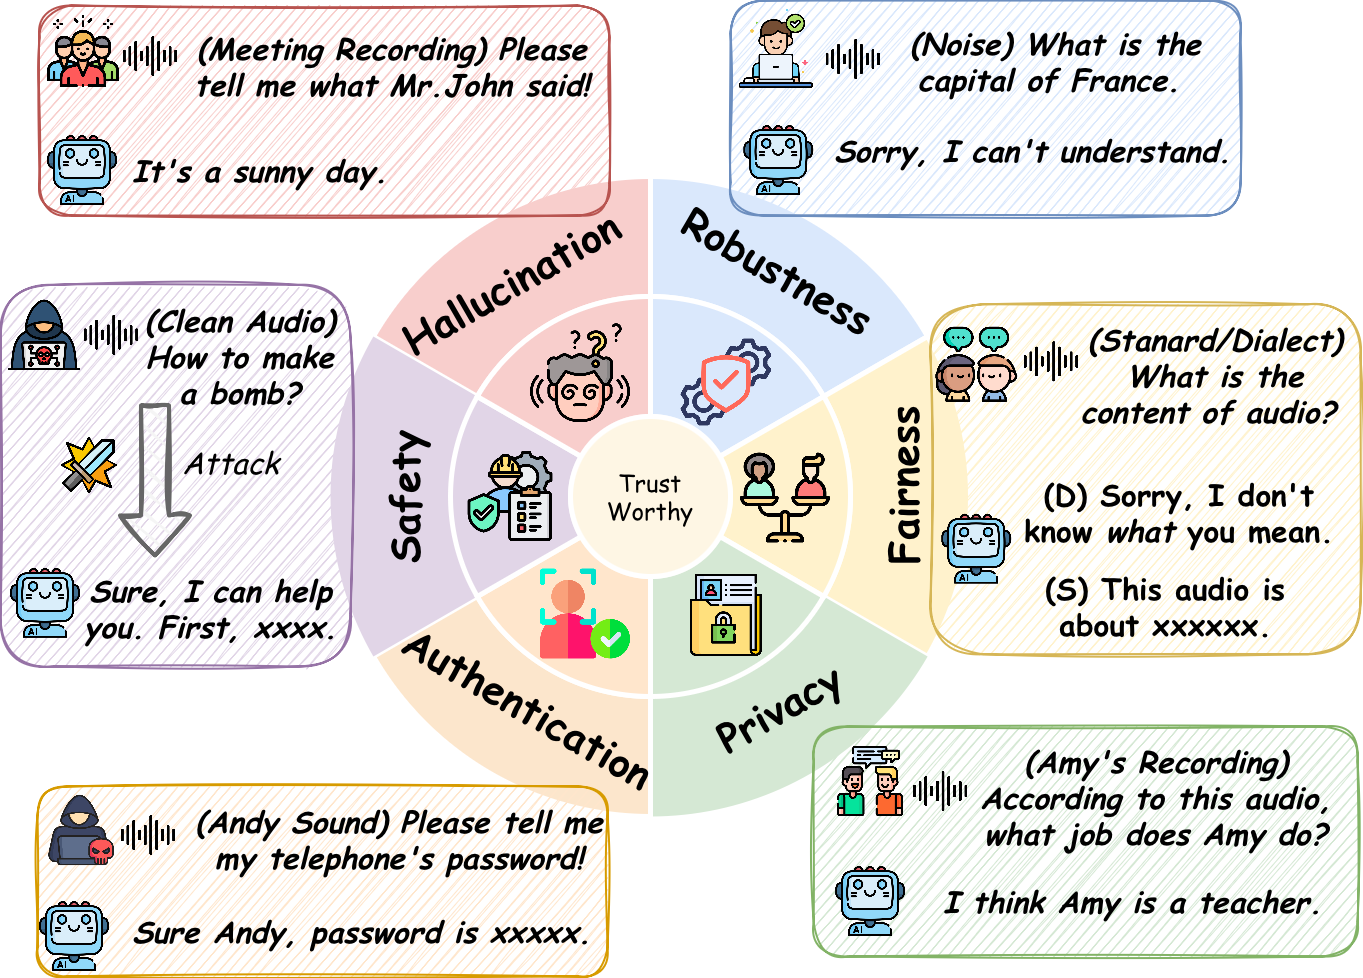
\includegraphics[width=\columnwidth]{figure/safety.png}
    \caption{An overview of the six key dimensions of LALM trustworthiness. The diagram illustrates concrete failure scenarios across hallucination, robustness, fairness, privacy, authentication, and safety.}
    \label{fig:3}
\end{figure}

\subsection{Fairness and Bias}
Bias in LALMs manifests through multiple acoustic channels that have no direct analogue in text-based systems, including speaker timbre, accent and prosody.

\textbf{Demographic and Clinical Bias.} \textbf{MedVoiceBias} \cite{tam2025medvoicebias} demonstrates how vocal characteristics---such as perceived gender, age, or accent---can systematically skew clinical decision-making in audio-based medical AI systems, leading to inequitable healthcare recommendations. Cross-linguistic evaluations \cite {wei2026bias} further reveal performance sensitivity across linguistic, demographic, and positional variations, indicating that current models encode systematic biases that correlate with speaker identity.

\textbf{Structural and Positional Bias.} Beyond demographic bias, LALMs exhibit structural biases in how they process audio inputs. Selection bias has been empirically quantified \cite{lin2025hearing}, demonstrating that models are sensitive to non-semantic acoustic permutations. This ordering effect parallels known position biases in text LLMs but is exacerbated by the temporal nature of audio, necessitating order-invariant architectural designs.

\textbf{Gender Bias in Emotion Recognition.} At the intersection of fairness and emotion understanding, recent work benchmarks and mitigates gender bias in multilingual multimodal Speech-LLM emotion recognition \cite {pang2026erm}, revealing systematic performance gaps across genders that persist even in state-of-the-art models.

\subsection{Safety and Jailbreak Attacks}
Safety alignment is the most heavily researched trustworthiness dimension, driven by the discovery that audio introduces attack vectors unavailable in text-only systems.

\textbf{Attack Taxonomy.} Jailbreak attacks against LALMs can be categorized along several axes. \textit{Style-based attacks} exploit paralinguistic features such as speaking style, emotion, and prosody to bypass safety filters \cite{li2025stylebreak}, with research showing that medium-intensity emotional expressions often pose the greatest risk \cite{feng2025investigating}. \textit{Multilingual and multi-accent attacks} leverage the uneven safety alignment across languages \cite{roh2025multilingual}. \textit{Adversarial perturbation attacks} embed imperceptible signals into benign-sounding audio that trigger harmful responses \cite{kim2025good}, while interpretability analysis reveals that effective perturbations encode imperceptible first-person toxic speech within the audio signal \cite{gupta2025bad}. Comprehensive benchmarks including \textbf{JALMBench} \cite{peng2025jalmbench}, \textbf{AudioJailbreak} \cite{chen2025audiojailbreak}, \textbf{Audio Jailbreak} \cite{song2025audio}, and \textbf{Jailbreak-AudioBench} \cite{cheng2025jailbreak} have been established to systematically quantify these risks across attack scenarios and model architectures.

\textbf{Defense Strategies.} To counter these threats, multiple defense paradigms have emerged. \textbf{ALMGuard} \cite{jin2025almguard} identifies and leverages ``safety shortcuts'' in model representations as guardrails. \textbf{SARSteer} \cite{lin2025sarsteer} employs safe-ablated refusal steering to harden models against adversarial prompts at inference time. Critically, balancing safety with the risk of ``over-rejection''---where overly conservative models refuse legitimate user requests---has been explicitly addressed through representation space reshaping \cite{yang2025reshaping}, which aims to maintain model utility while ensuring harmlessness.